\documentclass[a4paper]{article}
\usepackage{booktabs}
\usepackage{array}
\usepackage{wrapfig}
\usepackage{multirow}
\usepackage{tabularx}
\usepackage{graphicx}
\usepackage{pgf, tikz}
\usepackage[margin=0.375cm]{subcaption}
\usepackage{footnote}
% for tables i used minipage instead
%\makesavenoteenv{tabular}
%\makesavenoteenv{table}
\makesavenoteenv{figure}
\usepackage{amsmath}
\usepackage{amsthm}
\usepackage{amssymb}
\usepackage{mdframed}
\usepackage{csquotes}
\usepackage{polyglossia}
\usepackage{pifont}
\newcommand{\cmark}{\ding{51}}%
\newcommand{\xmark}{\ding{55}}%
\setdefaultlanguage{english}
\usepackage[style=alphabetic,minalphanames=3,maxbibnames=99]{biblatex}
\usepackage{hyperref}
\usepackage{cleveref}
\crefname{section}{\S}{\S\S}
\Crefname{section}{\S}{\S\S}

\addbibresource{references.bib}

\usetikzlibrary{arrows, automata}

\def\bitcoinA{%
  \leavevmode
  \vtop{\offinterlineskip %\bfseries
    \setbox0=\hbox{B}%
    \setbox2=\hbox to\wd0{\hfil\hskip-.03em
    \vrule height .3ex width .15ex\hskip .08em
    \vrule height .3ex width .15ex\hfil}
    \vbox{\copy2\box0}\box2}}

% reduce page count
\addtolength{\oddsidemargin}{-.875in}
\addtolength{\evensidemargin}{-.875in}
\addtolength{\textwidth}{1.75in}
\addtolength{\topmargin}{-.875in}
\addtolength{\textheight}{1.75in}

%\setlength{\belowcaptionskip}{-10pt}

\title{WabiSabi - Draft v0.3}
\author{Ádám Ficsór, Yuval Kogman, István András Seres}
\date{\today}

\begin{document}

\maketitle

\begin{abstract}
Bitcoin transfers value on a public ledger of transactions anyone can verify. Coin ownership is defined there in terms of public keys.
Despite potential use for private transfers, research has shown that users' activity can often be traced in practice. Businesses have been built on dragnet surveillance of Bitcoin users because of this lack of strong privacy, which harms its fungibility, a basic property of functional money.

Although the public nature of this design lacks strong guarantees for privacy, it does not rule it out.
A number of methods have been proposed to strengthen privacy. Among these is CoinJoin, which is an approach to structure transactions which adds ambiguity and breaks common assumptions that underlie heuristics used for surveillance.
Existing implementations of CoinJoin present a number of limitations which may partly explain the lack of their widespread adoption.

This work introduces \emph{WabiSabi}\footnote{The Japanese concept \emph{wabi-sabi} is an aesthetic world view which among other things emphasizes acceptance of imperfections, in our case Bitcoin's challenges for privacy, and an appreciation for simplicity and economy.}, a new protocol for centrally coordinated CoinJoin implementations utilizing keyed verification anonymous credentials and homomorphic value commitments. This improves earlier approaches which utilize blind signatures in both privacy and flexibility, enabling novel use cases and reduced overhead.
\end{abstract}

\section{Introduction}

Bitcoin transactions transfer funds by consuming unspent outputs of previous transactions as inputs to create new outputs. The protocol rules enforced by the network ensure that transactions do not arbitrarily inflate the money supply and that outputs are spent at most once. While some newer cryptocurrencies use more sophisticated approaches to define such rules, in Bitcoin the amounts as well as the specific outputs being spent are broadcast in the clear as part of the transaction. This presents significant challenges to transacting privately\footnote{In this work we restrict the discussion of Bitcoin privacy to that of public ledger transactions, but there are other considerations especially at the network layer. For a more comprehensive discussion see \url{https://en.bitcoin.it/wiki/Privacy}.} as shown already in some of the earliest academic studies of Bitcoin~\cite{reid2013analysis,ron2013quantitative,androulaki2013evaluating,ober2013structure,moeser2013inquiry,meiklejohn2013fistful}.

A fundamental requirement for electronic money is double spending prevention, and Bitcoin's main innovation was preventing double spending and illegal inflation without relying on a trusted authority and disintermediating transactions. This is in contrast to online e-cash schemes where a server authorizes transactions, or offline schemes where the identity of the double spender is revealed allowing the authority to intervene after the fact. Bitcoin's relative success suggests that the lack of trusted third parties factored more strongly in its adoption than the comparatively stronger privacy guarantees provided by the (possibly revocable) transaction  anonymity traditionally associated with e-cash~\cite{davida1997anonymity}.

These shortcomings in privacy affect Bitcoin users, both individuals and organizations, leaving casual users especially vulnerable since power to surveil and resist surveillance is unevenly distributed~\cite{rogaway2015moral}. Even without address reuse, which is pervasive, transactions still reveal some information. This makes clustering of outputs according to heuristics practical~\cite{harrigan2016unreasonable}, with wallets of some well known entities generally considered public knowledge. Exchanges complying KYC/AML requirements additionally must obtain and secure information that links transactions to personally identifying information.

The conditions for spending an output are specified in its \texttt{scriptPubKey}, typically requiring that the spending transaction be signed by a specific key. The signatures authorizing a transaction usually commit to the transaction in its entirety, making it possible for mutually distrusting parties to jointly create transactions without risking misallocation of funds: participants will only sign a proposed transaction after confirming that their desired outputs are included and the transaction is only valid when all parties have signed.

\subsection{Chaumian CoinJoin}

Chaumian CoinJoin~\cite{mizrahi2013blind,maxwell2013coinjoin,zerolink} is a privacy enhancing technique that uses the atomicity property of transactions and Chaumian blind signatures~\cite{chaum1983blind} to construct collaborative Bitcoin transactions, also known as CoinJoins. Participants connect to a server, known as the coordinator, and submit their inputs and outputs using different anonymity network identities. That alone would provide anonymity but since outputs are unconstrained it's not robust against malicious users who may disrupt the protocol by claiming more than their fair share. To mitigate this the coordinator provides blind signatures representing units of standard denominations in response to submitted inputs. By unblinding and presenting this valid signature, the coordinator is unable to link the signed output to specific inputs but can be still verify that an output registration is authorized.

The use of standard denominations in the resulting CoinJoin transaction obscures the relationship between individual inputs and outputs, making the origins of each output ambiguous. Unfortunately standard denominations limit the use of privacy-enhanced outputs for payments of arbitrary amounts and result in a change output which maintains a link to the non-private input.

\subsection{Limitations of Wasabi}\label{sec:limitations}
In this work, we aim to improve on ZeroLink~\cite{zerolink} as implemented by Wasabi, the most popular Chaumian CoinJoin implementation for Bitcoin. We identify several privacy shortcomings and inefficiencies of Wasabi CoinJoins. Some metrics comparing Wasabi, Samourai and other apparent CoinJoin transactions are provided. The ``Other'' category includes JoinMarket\footnote{\url{https://github. com/JoinMarket-Org/joinmarket}}, but also has an inherent false positive error given these transactions are identified heuristically.

\subsubsection{Denominations}

Due to the nature of blind signatures, mixed outputs of Wasabi CoinJoins are restricted to fixed set of multiples of a base denomination\footnote{Approximately $0.1$\bitcoinA{}}. This creates friction when sending or receiving arbitrary amounts of Bitcoin, as using fixed denomination generally creates change, both when mixing and when spending mixed outputs.

We define \emph{CoinJoin inefficiency} as the fraction of non-mixed change outputs in a CoinJoin transaction, see \cref{fig:cjinefficiency}.

\begin{figure}[h!]
    \centering
    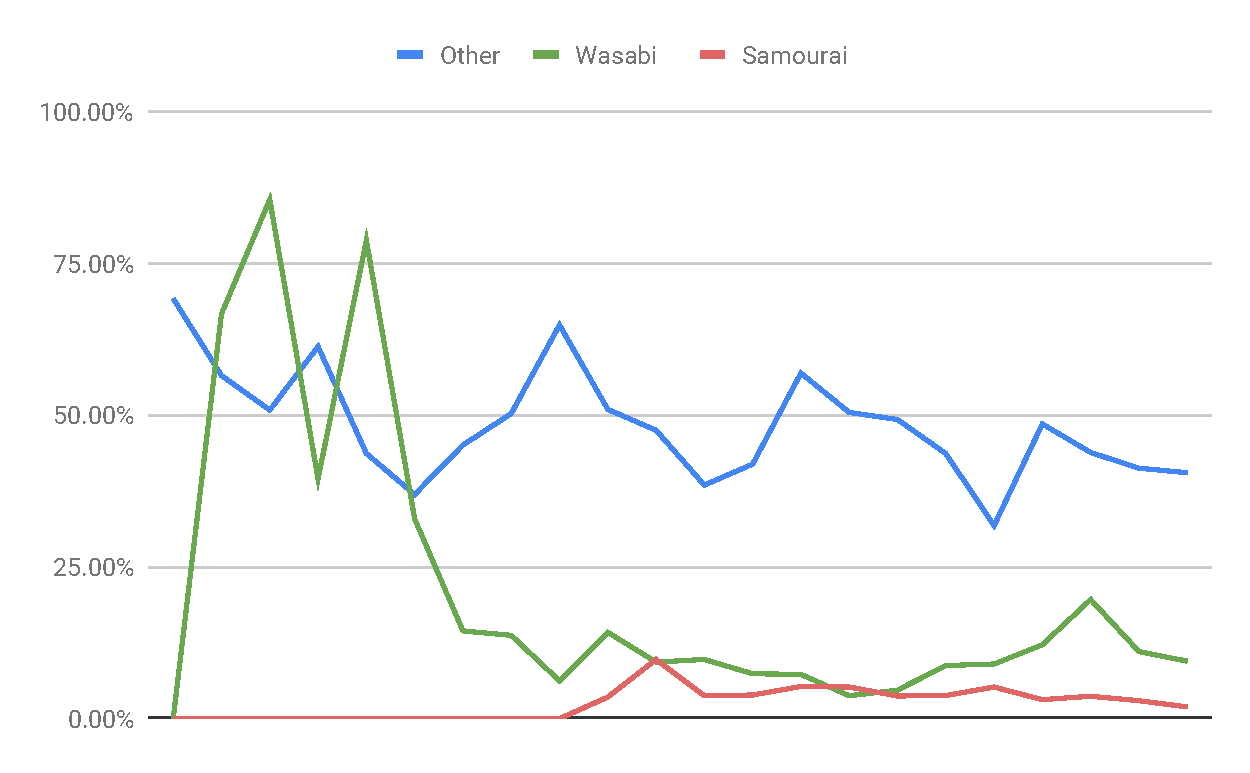
\includegraphics[scale=0.4]{Figures/CJInefficiency.pdf}
    \caption{CoinJoin inefficiency of various privacy-focused Bitcoin wallets.}
    \label{fig:cjinefficiency}
\end{figure}

\subsubsection{Minimum denomination}

In order to participate, a user's combined input amount must be greater or equal to the base denomination.\footnote{The observed base denominations in Wasabi's CoinJoins are usually slightly higher than the announced, agreed upon base denomination. Thus participants sometimes get back slightly more value in the CoinJoins than they put in.} We observe, that considerable portion of CoinJoin inputs are less than this minimum denomination, see \cref{fig:minimumdenomination}.

\begin{figure}[h!]
    \centering
    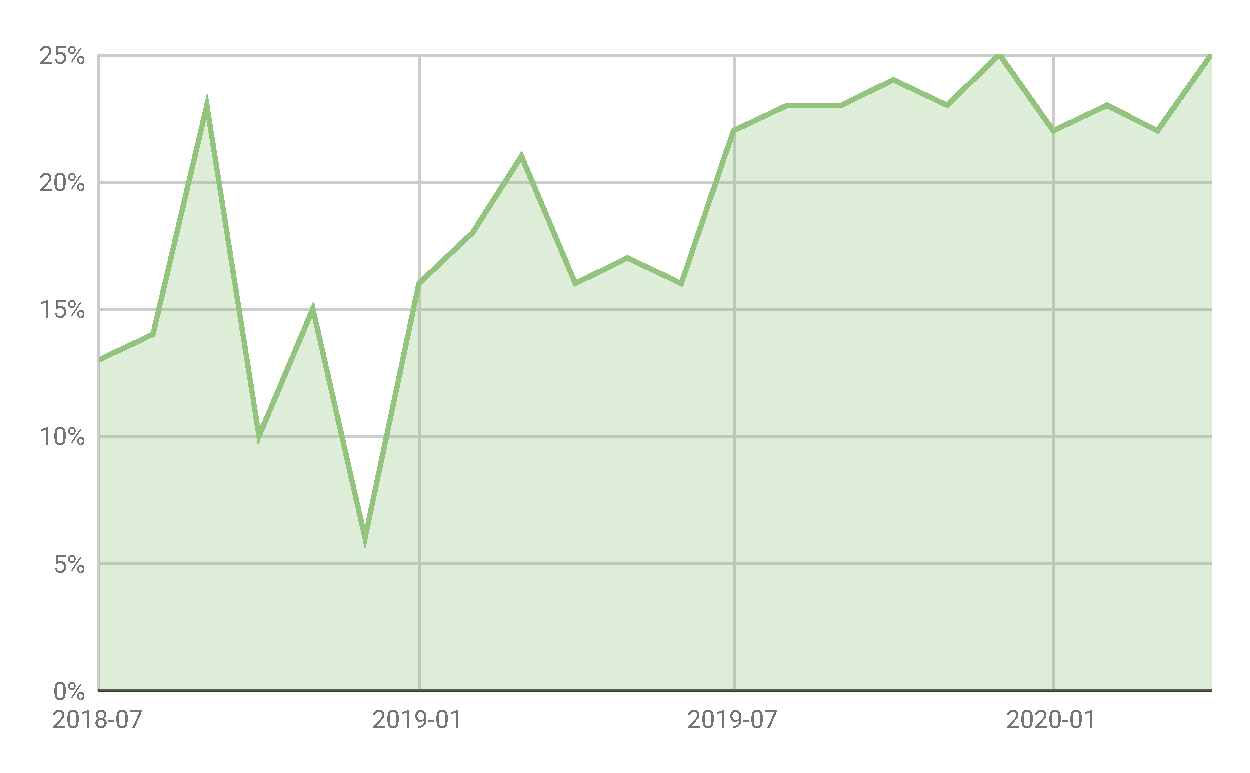
\includegraphics[scale=0.4]{Figures/SmallValueInputsWasabi.pdf}
    \caption{Fraction of inputs with value smaller than the minimum denomination in Wasabi CoinJoin transactions.}
    \label{fig:minimumdenomination}
\end{figure}

Even when users are able to provide several smaller value inputs with total value greater than the minimum denomination, the coordinator knows those inputs belong to the same user. In an ideal mixing protocol the coordinator should not obtain more information than the already available public ledger data by coordinating the CoinJoin transaction. This information removes many degrees of freedom when assigning non-derived sub-transactions~\cite{maurer2017anonymous} or link probability~\cite{laurentmt2015bitcoin}, reducing intrinsic ambiguity as well as the computational cost when evaluating potential links.

Furthermore if users consolidate coins before the CoinJoin in an additional transaction in order to be able to participate in a CoinJoin, then this link is revealed publicly based on the common input ownership heuristic~\cite{meiklejohn2013fistful}.

\subsubsection{Varying denominations} Since users pay mining and coordination fees the denominations are gradually reduced between rounds of consecutive CoinJoins in order to make it possible for users to mix several times without providing additional inputs. This introduces a perverse incentive to minimize coordination fees by remixing in quick succession in order, resulting in a smaller anonymity set than with time-staggered remixes.

\subsubsection{Block-space efficiency}

The rigidity of the current transaction structure, i.e. fixed denominations, constrains users' unspent transaction output set structure as well. These limitations force users to consolidate their coins (see \cref{fig:postmixmerging}) and create additional intermediate outputs with constrained amounts when interspersing CoinJoin transactions with transactions that send or receive value.

\begin{figure}[h!]
    \centering
    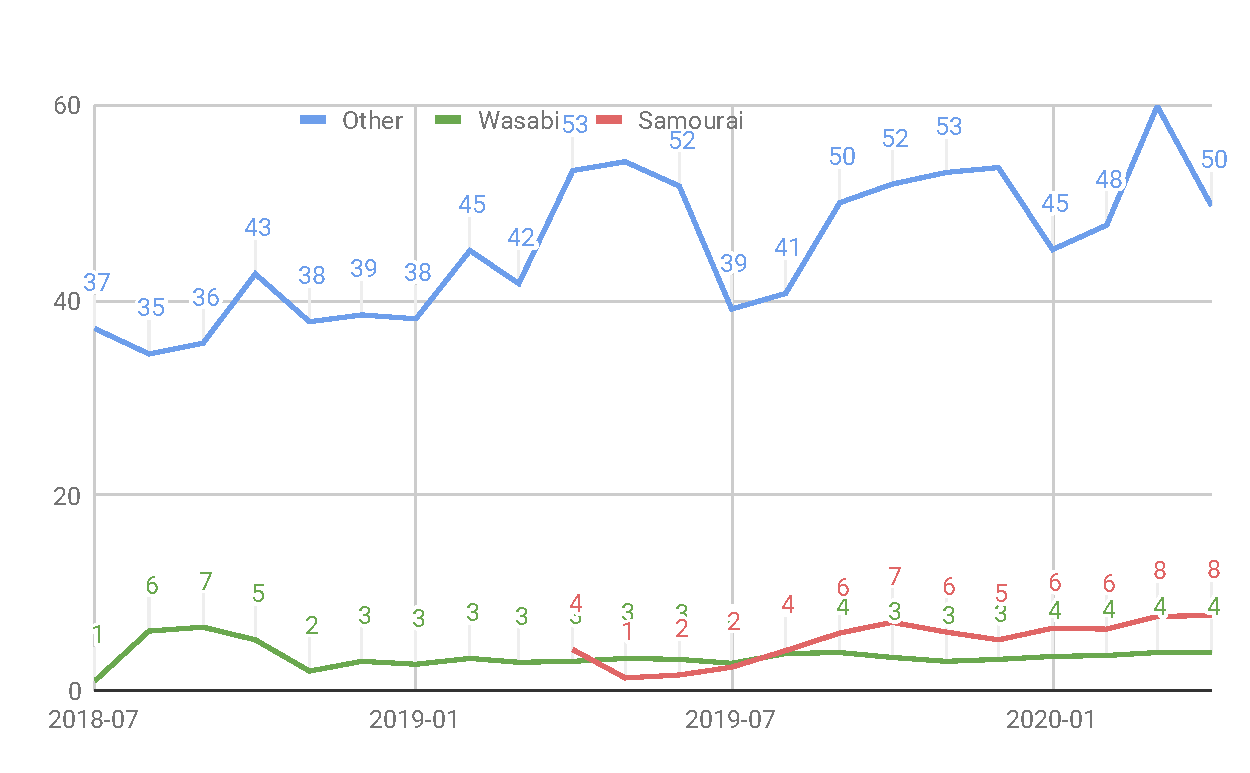
\includegraphics[scale=0.4]{Figures/postMixInputMerging.pdf}
    \caption[]{Average number of inputs from the first post-mix transactions in various CoinJoin schemes.\footnote{The large figures for other CoinJoin-like transactions suggests false positives in our identification.}}
    \label{fig:postmixmerging}
\end{figure}

\subsubsection{Lack of privacy-enhanced payments} Currently Wasabi supports neither payments from a CoinJoin, nor payments in a CoinJoin. Payments from a CoinJoin would protect sender privacy and improve efficiency by requiring fewer intermediate outputs. Payments within a CoinJoin would protect both sender and receiver privacy, and since they are a form of PayJoin\footnote{\url{https://en.bitcoin.it/wiki/PayJoin}} it would also improve privacy by introducing degrees of freedom in the interpretation of CoinJoins.

\subsection{Our Contribution}

We present WabiSabi, a generalization of Chaumian CoinJoin based on a keyed-verification anonymous credentials (KVAC) scheme~\cite{chase2019signal}. The use of KVACs replaces blind signatures' standard denominations with homomorphic amount commitments, similar to Confidential Transactions~\cite{maxwell2016confidential}, where the sum of any participant's outputs does not exceed that of their inputs while hiding the underlying values from the coordinator. In addition to being more flexible this improves privacy compared to blind signatures and standard denominations, since smaller inputs can be combined and change outputs created with the same unlinkability guarantees as those of standard denominations when using blind signatures\footnote{Note that the cleartext amounts appearing in the final transaction might still link individual inputs and outputs.}. WabiSabi builds on a successfully deployed and proven approach, aiming to reduce barriers to further adoption~\cite{dingledine2006anonymity} by removing restrictions and strengthening unlinkability.

WabiSabi can be instantiated to construct a variety of CoinJoin transaction structures that depart from the standard output denomination convention, as in SharedCoin\footnote{\url{https://github.com/sharedcoin/Sharedcoin}} and CashFusion\footnote{\url{https://github.com/cashshuffle/spec}} style transactions and Knapsack~\cite{maurer2017anonymous} mixing. Payments from CoinJoin transactions are possible, as are payments within them, effectively a multiparty PayJoin that trades the steganographic properties for improved privacy from counterparties. Additionally, restrictions on consolidation of inputs can be removed, and there are opportunities for reducing unmixed change and relaxing minimum required denominations, and improved block space efficiency.

The rest of this paper is organized as follows. In \cref{sec:preliminaries} we provide some background on our applied cryptographic building blocks. In \cref{sec:overview} we introduce our protocol, WabiSabi, at a high-level, while in \cref{sec:details} we describe in-depth the cryptographic details of WabiSabi. In \cref{sec:securitayandprivacy} we argue about the security and privacy of WabiSabi.
We review related work in \cref{sec:relatedwork}. Finally, we conclude our paper in \cref{sec:conclusion}.

\section{Preliminaries}\label{sec:preliminaries}

Hereby we give an informal and high-level description of applied cryptographic primitives. In the following the security parameter is denoted as $\lambda$.

\subsection{Commitment schemes}
A commitment scheme allows one to commit to a chosen message while preventing them from changing the message after publishing the commitment. Secure commitments hide the chosen message until they are opened. We assume Pedersen commitments throughout this work.

\begin{description}

\item[$\mathsf{Commit}(m,r)\mapsto{}\mathcal{C}$:] generate a commitment $\mathcal{C}$ to message $m$ using randomness $r$.

\item[$\mathsf{OpenCom}(\mathcal{C},m,r)\mapsto{}\{\mathit{True},\mathit{False}\}$:] verify the correctness of the opening of a commitment by checking $\mathcal{C}\stackrel{?}{=}\mathsf{Commit}(m,r)$. If equality holds the algorithm outputs $\mathit{True}$, otherwise $\mathit{False}$.

\end{description}.

\subsection{MAC}
A message authentication code (MAC) ensures the integrity of a message and consists of the following three probabilistic polynomial-time algorithms:

\begin{description}

\item[$\mathsf{GenMACKey}(\lambda)\mapsto{}{\mathsf{sk}}$:] generate a secret key $\mathsf{sk}$ for MAC generation and verification.

\item[$\mathsf{MAC}_{\mathsf{sk}}(m)\mapsto{}t$:] generate a tag $t$ on a message $m$ using secret key $\mathsf{sk}$.

\item[$\mathsf{VerifyMAC}_{\mathsf{sk}}(m,t)\mapsto{}\{\mathit{True},\mathit{False}\}$:] verify that tag $t$ is valid for message $m$ using secret key $\mathsf{sk}$.

\end{description}

One might intuitively think of a MAC as the symmetric-key counterpart of digital signatures. They both have the same goals and similar security requirements, however a MAC requires a secret rather than public key to verify.

\subsection{Zero-knowledge proofs of knowledge}
A very high-level, and hence somewhat imprecise, description of zero-knowledge proofs is provided. This protocol involves a prover and a verifier. A prover wishes to prove that a relation $\mathcal{R}$ holds with respect to a secret input $w$, called witness, and public input $x$. Specifically, the prover wants to prove that $(x, w) \in \mathcal{R}$ without revealing anything about $w$.

\begin{description}
\item[$\mathsf{Prove}_{\mathcal{R}}(x,w)\mapsto{}\pi$:] Given $x$ and the private witness $w$ the prover generates a proof $\pi$. For the specific outputs of $\mathsf{Prove}$ we use the notation of~\cite{camenisch1997proof}, with the witness and statement: $\pi = \operatorname{PK}\{ (w) : (w, x) \in \mathcal{R} \}$.

\item[$\mathsf{Verify}_{\mathcal{R}}(x,\pi)\mapsto{}\{\mathit{True},\mathit{False}\}$:] The verifier is given the proof $\pi$ and $x$ with which they determine whether the prover knows a secret $w$ such that $(w,x) \in \mathcal{R}$ holds.
\end{description}

\section{Overview} \label{sec:overview}
In this section we provide a high-level overview of our WabiSabi protocol.
\subsection{Phases}

A CoinJoin round consists of an Input Registration, an Output Registration and a Transaction Signing phase. To defend against Denial of Service attacks it is important to ensure the inputs of users who do not comply with the protocol are identified so these inputs can be excluded from the following rounds in order to ensure completion of the protocol.

\begin{enumerate}
    \item While identifying non-compliant inputs during Input Registration phase is trivial, there is no reason to issue penalties at this point.
    \item Identifying non-compliant inputs during Output Registration phase is not possible, thus this phase always completes and progresses to the Signing phase.
    \item During Signing phase, inputs which are not signed are non-compliant inputs and they shall be issued penalties.
\end{enumerate}

The cryptography in WabiSabi ensures honest participants always agree to sign the final CoinJoin transaction if the coordinator is honest. Anonymous credentials allow the coordinator to verify that amounts of each user's output registrations are funded by input registrations without learning specific relationships between inputs and outputs.

\subsection{Credentials}

The coordinator issues anonymous credentials which authenticate attributes in response to registration requests. We use keyed-verification anonymous credentials (introduced in~\cite{chase2014algebraic}), in particular the scheme from~\cite{chase2019signal} which supports group attributes (attributes whose value is an element of the underlying group $\mathbb{G}$). A user can then prove possession of a credential in zero knowledge in a subsequent registration request, without the coordinator being able to link it to the registration from which it originates.

In order to facilitate construction of a CoinJoin transaction while protecting the privacy of participants, we instantiate the scheme with a single group attribute $M_a$ which encodes a confidential Bitcoin amount as a Pedersen commitment. These commitments are never opened. Instead, properties of the values they commit to are proven in zero knowledge, allowing the coordinator to validate requests made by honest participants. In ideal circumstances the coordinator would not learn anything beyond what can be learned from the resulting CoinJoin transaction but despite the unlinkability of the credentials timing of requests or connectivity issues may still reveal information about links.

\subsection{Registration}

To aid intuition we first describe a pair of protocols, where credentials are issued during input registration, and then then presented at output registration. $k$ denotes the number of credentials used in registration requests, and $a_{\mathit{max}} = 2^{51}-1$ constrains the range of amount values\footnote{$\log_2(2099999997690000) \approx 50.9$}. For better privacy and efficiency these are then generalized into a unified protocol used for both input and output registration, where every registration involves both presentation and issuance of credentials. This protocol is described in detail in \cref{sec:details}.

In order to maintain privacy clients must isolate registration requests using unique network identities. A single network identity must not expose more than one input or output, or more than one set of requested or presented credentials.

For fault tolerance, request handling should be idempotent, allowing a client to retry a failed request without modification using a fresh network identity or one which was previously used to attempt that request.

\subsubsection{Input Registration}

\begin{figure}[h!]
    \begin{mdframed}
    \begin{enumerate}
        \item The user sends $k$ credential requests with accompanying range and sum proofs to the coordinator:  $((M_{a_i},\pi^{\textit{range}}_{i})^{k}_{i=1},\pi^{sum},a_{\textit{in}})$.
        \item The coordinator verifies the received proofs. If they are not verified it aborts the protocol, otherwise it issues $k$ MACs on the requested attributes $(\mathsf{MAC}_\mathsf{sk}(M_{a_i}), \pi_i^{\mathrm{iparams}})^{k}_{i=1}$.
    \end{enumerate}

\end{mdframed}
    \caption{Input Registration protocol}
    \label{fig:inputreg}
\end{figure}

The user submits an input of amount $a_{\mathit{in}}$ along with $k$ group attributes, $(M_{a_i})$.
She proves in zero knowledge that the sum of the requested sub-amounts is equal to $a_{\mathit{in}}$ and that the individual amounts are positive integers in the allowed range.

The coordinator verifies the proofs, and issues $k$ MACs on the requested attributes, along with a proof of correct generation of the MAC, as in \textit{Credential Issuance} protocol of \cite{chase2019signal}.

\subsubsection{Output Registration}

\begin{figure}[h!]
    \begin{mdframed}
    \begin{enumerate}
        \item The user sends $k$ randomized commitments, a proof of a valid MAC for the corresponding non-randomized commitments, serial numbers with a proof of their validity, and finally a proof of the sum of the amounts: $((C_{a_i},\pi_{i}^{\textit{MAC}},S_i,\pi_i^{\textit{serial}})^{k}_{i=1}, \pi^{\textit{sum}}, a_{\textit{out}})$.
        \item The coordinator verifies proofs and registers requested output iff. all proofs are valid and the serial numbers have not been used before.
    \end{enumerate}
\end{mdframed}
    \caption{Output Registration protocol}
    \label{fig:outputreg}
\end{figure}

To register her output the user randomizes the attributes and generates a proof of knowledge of $k$ valid credentials issued by the coordinator.

Additionally, she proves the serial number is valid. These serial numbers are required for double spending protection, and must be correspond but unlinkable to a specific $M_a$.

Finally, she proves that the sum of her randomized amount attributes $C_a$ matches the requested output amount $a_{\mathit{out}}$, analogously to input registration.\footnote{Note that there is no need for range proofs, since amounts have been previously validated.}

She submits these proofs, the randomized attributes, and the serial numbers. The coordinator verifies the proofs, and if accepted the output will be included in the transaction.

\subsubsection{Unified Registration}\label{sec:unified}

In order to increase flexibility in a dynamic setting, where a user may not yet know her desired output allocations during input registration, and to allow setting a small\footnote{Specifically, $2 \le k \le 10 \approx \log_2\left(\frac{\mathtt{MAX\_STANDARD\_TX\_WEIGHT} - 58}{274 + 124}\right)$ the maximum number of participants, because although $k=1$ suffices for flexibility it limits parallelism, leaking privacy by temporal fingerprinting. The limit on participant count is because 274 and 124 are the minimum weight units required for a participant with only a single input and output, and 58 is the shared per transaction overhead.} value of $k$ as a protocol level constant to reduce privacy leaks, we can generalize input and output registration into a single unified protocol for use in both phases, which also supports reissuance. For complete definitions see \cref{sec:details}.

\begin{figure}[h!]
    \begin{mdframed}
    \begin{enumerate}
        \item During both input and output registration phases the user submits:
        \begin{itemize}
            \item $k$ credential requests with accompanying range and sum proofs to the coordinator:  $(M_{a_i},\pi^{\textit{range}}_{i})^{k}_{i=1}$
            \item $k$ randomized commitments, proofs of valid credentials issued for the corresponding non-randomized commitments, serial numbers, and proofs of their validity: $(C_{a_i},\pi_{i}^{\mathit{MAC}},S_i,\pi_i^{\textit{serial}})^{k}_{i=1}$
            \item A balance $\Delta_{a}$ and a proof of its correctness $\pi^{\textit{sum}}$
            \item If $\Delta_{a} \ne 0$, an input or output with value $|\Delta_{a}|$.
        \end{itemize}
        \item The coordinator verifies the received proofs, and that the serial numbers have not been used before, and depending on the current phase, $\Delta_{a} \geq 0$ (input) or $\Delta_{a} \leq 0$ (output). If it accepts, it issues $k$ MACs on the requested attributes $(\mathsf{MAC}_\mathsf{sk}(M_{a_i}), \pi_i^{\mathrm{iparams}})^{k}_{i=1}$, and if $\Delta_{a} \ne 0$, registers the input or output with value $|\Delta_{a}|$.
    \end{enumerate}
    \end{mdframed}
    \caption{Unified Registration protocol}
    \label{fig:reissue}
\end{figure}

The user submits $k$ valid credentials and $k$ credential requests, where the sums of the underlying amount commitments must be balanced (\cref{fig:reissue}).

\begin{figure}[h!]
  \begin{mdframed}
    \begin{enumerate}
    \item During input registration phase the user submits $k$ credential requests:  $(M_{a_i},\pi^{\mathit{null}}_{i})^{k}_{i=1}$
    \item The coordinator verifies the received proofs. If it accepts, it issues $k$ MACs on the requested attributes $(\mathsf{MAC}_\mathsf{sk}(M_{a_i}), \pi_i^{\mathrm{iparams}})^{k}_{i=1}$.
    \end{enumerate}
  \end{mdframed}
  \caption{Credential bootstrapping protocol}
  \label{fig:bootstrap}
\end{figure}

To prevent the coordinator from being able to distinguish between initial vs. subsequent input registration requests (which may merge amounts) credential presentation should be mandatory. Initial credentials can be obtained with an auxiliary bootstrapping operation (\cref{fig:bootstrap}).

\subsection{Signing phase}

The user fetches the finalized but unsigned transaction from the coordinator. If it contains the outputs she registered she will sign her inputs and submit each signature separately using the network identity used for that input's registration.

\subsection{Examples}\label{sec:examples}

% todo sub figures

To illustrate the above protocols, \cref{fig:ex1,fig:ex2} show how a user might register inputs and outputs when credentials are only presented during the output registration phase and \cref{fig:ex3,fig:ex4} show the unified protocol, when credentials are both presented and requested in every registration request.

Registration requests are depicted as vertices labeled with $\Delta_a$, a double stroke denoting output registrations. A credential is an edge from the registration in which it was requested to the registration where it was presented, also labeled with the amount. The vertex's label must be equal to the balance of the labels of its incoming edges and its outgoing edges. Note that edges and their labels are only known to the owners of the credentials. For simplicity we omit credentials with zero value.

\begin{figure}[h!]
  \centering
  \begin{subfigure}{.45\linewidth}
  \centering
  \begin{tikzpicture}[
    auto,
    node distance = 1cm,
    shorten  >=1pt,
    ]

    \tikzstyle{every state}=[
    draw = black,
    thick,
    fill = white,
    ]

    \node[state] (i) {10};
    \node[accepting,state] (o1) [above right of=i, xshift=1.75cm] {7};
    \node[accepting,state] (o2) [below right of=i, xshift=1.75cm] {3};

    \path[->] (i) edge node {\tiny{7}} (o1);
    \path[->] (i) edge node {\tiny{3}} (o2);
  \end{tikzpicture}
  \caption{Alice wants to spend an input of amount 10 and create two outputs with amounts 7 and 3 (e.g. a payment and change)}
  \label{fig:ex1}
\end{subfigure}
 \begin{subfigure}{.45\linewidth}
  \centering
  \begin{tikzpicture}[
    auto,
    node distance = 1.5cm,
    shorten  >=1pt,
    semithick,
    ]

    \tikzstyle{every state}=[
    draw = black,
    thick,
    fill = white,
    ]

    \node[state] (i1) {6};
    \node[state] (i2) [below of=i1] {4};
    \node[accepting,state] (o1) [right of=i1, xshift=1.75cm] {7};
    \node[accepting,state] (o2) [right of=i2, xshift=1.75cm] {3};

    \path[->] (i1) edge node {\tiny{6}} (o1);
    \path[->] (i2) edge node {\tiny{1}} (o1);
    \path[->] (i2) edge node {\tiny{3}} (o2);
  \end{tikzpicture}
  \caption{Alice wants to combine her inputs of amounts 6 and 4 and register two outputs as in \cref{fig:ex1}.}
  \label{fig:ex2}
\end{subfigure}

\begin{subfigure}{.45\linewidth}
  \centering
  \begin{tikzpicture}[
    auto,
    node distance = 1.75cm,
    shorten  >=1pt,
    semithick,
    ]

    \tikzstyle{every state}=[
    draw = black,
    thick,
    fill = white,
    ]

    \node[state] (i1) {6};
    \node[state] (i2) [right of=i1] {4};
    \node[accepting,state] (o1) [above right of=i2, xshift=1cm] {7};
    \node[accepting,state] (o2) [below right of=i2, xshift=1cm] {3};

    \path[->] (i1) edge node {\tiny{6}} (i2);
    \path[->] (i2) edge node {\tiny{7}} (o1);
    \path[->] (i2) edge node {\tiny{3}} (o2);
  \end{tikzpicture}
  \caption{Alice wants to spend two inputs and register two outputs using the unified protocol, which allows her to present the credential from her first input registration when registering her second input to combine the amounts.}
  \label{fig:ex3}
  \end{subfigure}
\begin{subfigure}{.45\linewidth}
  \centering
  \begin{tikzpicture}[
    auto,
    node distance = 1.75cm,
    shorten  >=1pt,
    semithick,
    ]

    \tikzstyle{every state}=[
    draw = black,
    thick,
    fill = white,
    ]

    \node[state] (i1) {$6_A$};
    \node[state] (i2) [right of=i1] {$4_A$};
    \node[state] (i3) [below right of=i2] {$4_B$};
    \node[accepting,state] (o1) [above right of=i2, xshift=1.5cm] {$3_A$};
    \node[accepting,state] (o2) [below of=o1] {$10_B$};
    \node[accepting,state] (o3) [below of=o2] {$1_B$};

    \path[->] (i1) edge node {\tiny{6}} (i2);
    \path[->] (i2) edge node {\tiny{7}} (i3);
    \path[->] (i2) edge node {\tiny{3}} (o1);
    \path[->] (i3) edge node {\tiny{10}} (o2);
    \path[->] (i3) edge node {\tiny{1}} (o3);
  \end{tikzpicture}
  \caption{Alice wants to pay Bob, who is also participating in the protocol. Alice combines her amounts at input registration and reveals a credential corresponding to the payment amount to Bob. Bob presents this credential in his own input registration. Alice registers a change output, and Bob registers two outputs. Only Alice knows the details of the request in which the credential labeled 7 was issued and only Bob knows where it was presented, but both know the amount.}
  \label{fig:ex4}
  \end{subfigure}
  \caption{Credential usage examples}
\end{figure}

\section{WabiSabi Credentials}\label{sec:details}

In this section we provide the details of the unified protocol (\cref{sec:unified}) and its use of the KVAC scheme introduced in~\cite{chase2019signal}. Following that work our protocol is defined over an Abelian group \(\mathbb{G}\) of prime order \(q,\) written in multiplicative notation.
$\mathsf{HashTo\mathbb{G}} : \{0,1\}^{*} \mapsto \mathbb{G}$ is a function from strings to group elements, based on a cryptographic hash function\cite{fouque2012indifferentiable}.

We require the following fixed set of group elements for use as generators with different purposes:
\[
\underbrace{G_{w}, G_{w^{\prime}}, G_{x_{0}}, G_{x_{1}}, G_{V}}_{\mathsf{MAC} \text{~and~} \mathsf{Show}}
\qquad
\underbrace{G_a}_{\text{attributes}}
\qquad
\underbrace{G_g, G_h}_{\text{commitments}}
\qquad
\underbrace{G_s}_{\text{serial numbers}}
\]
chosen so that nobody knows the discrete logarithms between any pair of them, e.g. $G_h = \mathsf{HashTo\mathbb{G}}(``\texttt{h}")$.

Our notation deviates slightly from \cite{chase2019signal}, in that we subscript the attribute generators $G_{y_i}$ as $G_a$ instead of using numerical indices, and we require two additional generators $G_g$ and $G_h$ for constructing the attribute $M_a$ as a Pedersen commitment.

As with the generator names, we modify the names of the attribute related components of the secret key
$\mathrm{sk} = (w, w^{\prime}, x_{0}, x_{1}, y_{a}) \in_R {\mathbb{Z}_q}^5$
according to our fixed set of group attributes.

The coordinator parameters
$\mathit{iparams} =  (C_{W}, I)$
are computed as:
\[
C_{W}={G_w}^{w} {G_{w^\prime}}^{w^\prime}
\quad
I=\frac{G_{V}}{{G_{x_0}}^{x_0} {G_{x_1}}^{x_1} {G_a}^{y_a} }
\]
and published as part of the round metadata and are used by the coordinator to prove correctness of issued MACs, and by the users to prove knowledge of a valid MAC.

\subsection{Credential Requests}

For each $i \in [1, k]$ the user chooses an amount $a_i \mid 0 \leq a_i < a_{\mathit{max}}$ subject to the constraints of the balance proof (\cref{balance}). She commits to the amount with randomness $r_i \in_R \mathbb{Z}_q$, and these commitments are the attributes of the requested credentials:
\[ M_{a_i}={G_h}^{r_i}{G_g}^{a_i} \]

For each amount $a_i$ she also computes a range proof which ensures there are no negative values:
\[
\pi^{\mathit{range}}_i = \operatorname{PK}\left\{\left(a_i, r_i \right) :
M_{a_i} = {G_h}^{r_i}{G_g}^{a_i}
\land
0 \leq a_i < a_{\mathit{max}} \right\}
\]

In credential bootstrap requests the range proofs can be replaced with simpler proofs of $a_i = 0$:
\[
  \pi^{\mathit{null}}_i = \operatorname{PK}\left\{ \left( r_i\right) :
    M_{a_i} = {G_{h}}^{r_i}
  \right\}
\]

We note that if Bulletproofs~\cite{bunz2018bulletproofs} are utilized for the range proofs $\pi^{\textit{range}}_i$ a combined proof will significantly decrease the communication overhead and that some implementations perform the $\pi^{\mathrm{null}}$ optimization already.

\subsection{Credential Issuance}

If the coordinator accepts the requests (see \cref{presentation,serial,balance}), it registers the input or output if one is provided, and for each $i \in [1,k]$ it issues a credential by responding with
$(t_i, V_i) \in \mathbb{Z}_q \times \mathbb{G}$,
which is the output of
$\mathsf{MAC}_{\mathsf{sk}}(M_{a_i})$,
where:
\[
  t_i \in_{R} \mathbb{Z}_{q}
  \qquad
  U_i = \mathsf{HashTo\mathbb{G}}(t_i)
  \qquad
  V_i={G_w}^{w} {U_i}^{x_{0}+x_{1} t_i}{M_{a_i}}^{y_a}
\]


To rule out tagging of individual users the coordinator must prove knowledge of the secret key, and that $(t_i, U_i, V_i)$ are correct relative to $\mathit{iparams}=(C_{W}, I)$:

\begin{align*}
  \pi_{i}^{\mathit{iparams}}=\operatorname{PK}\{ & (w, w^{\prime}, x_{0}, x_{1}, y_a): \\
                                                 &C_{W}={G_{w}}^{w} {G_{w^{\prime}}}^{w^\prime} \land \\
                                                 &I=\frac{G_{V}}{{G_{x_{0}}}^{x_0} {G_{x_1}}^{x_1} {G_a}^{y_a}}  \land \\
                                                 &V_i={G_w}^{w}{U_i}^{x_{0}+x_{1}t_i} {M_{a_i}}^{y_a}
                                                   \}
\end{align*}

\subsection{Credential Presentation}\label{presentation}

The user chooses $k$ unused credentials issued in prior registration requests, i.e. valid MACs $(t_i,V_i)_{i=1}^k$ on attributes $(M_{a_i})_{i=1}^k$.

For each credential $i \in [1, k]$ she executes the $\mathsf{Show}$ protocol described in~\cite{chase2019signal}:

\begin{enumerate}

\item She chooses
$z_i \in_{R} \mathbb{Z}_{q}$, and computes
$z_{0_i}=-{t_i} {z_i} (\bmod q)$
and the randomized commitments:
\begin{align*}
C_{a_i}     &= {G_a}^{z_i} M_{a_i} \\
C_{x_{0_i}} &= {G_{x_0}}^{z_i} {U_i} \\
C_{x_{1_i}} &= {G_{x_1}}^{z_i} {U_i}^{t_i} \\
C_{V_i}     &= {G_V}^{z_i} V_i
\end{align*}

\item To prove to the coordinator that a credential is valid she computes a proof:
\begin{align*}
\pi_{i}^{\mathit{MAC}}=\operatorname{PK}\{
& (z_i, z_{0_i},t_i): \\
& Z_i =I^{z_i} \land \\
& C_{x_{1_i}} = {C_{x_{0_i}}}^{t_i} {G_{x_0}}^{z_{0_i}} {G_{x_1}}^{z_i} \}
\end{align*}
which implies the following without allowing the coordinator to link $\pi_{i}^\mathit{MAC}$ to the underlying attributes $(M_{a_i})$:
\[
\mathsf{Verify}((C_{x_{0_i}}, C_{x_{1_i}}, C_{V_i}, C_{a_i}, Z_i), \pi_i^{\mathit{MAC}})
\iff
\mathsf{VerifyMAC}_{\mathsf{sk}}(M_{a_i})
\]

\item She sends $(C_{x_{0_i}}, C_{x_{1_i}}, C_{V_i}, C_{a_i},\pi_i^{\mathit{MAC}})$ and the coordinator computes:
\[
Z_i=\frac{C_{V_i}}{{G_w}^w {C_{x_{0_i}}}^{x_0} {C_{x_{1_i}}}^{x_{1}}
{C_{a_i}}^{y_a}
}
\]
using its secret key (independently of the user's derivation), and verifies $\pi_i^{\mathit{MAC}}$.

\end{enumerate}

\subsection{Double-spending prevention using serial numbers}\label{serial}

The user proves that the group element $S_i = {G_s}^{r_i}$, which is used as a serial number, was generated correctly with respect to $C_{a_i}$:
\[ \pi_{i}^{\mathit{serial}}=\operatorname{PK}\{ (z_i,a_i,r_i): S_i = {G_s}^{r_i} \land C_{a_i} = {G_a}^{z_i}{G_h}^{r_i}{G_g}^{a_i} \} \]

The coordinator verifies $\pi_{i}^{\mathit{serial}}$ and checks that the $S_i$ has not been used before (allowing for idempotent registration).

Note that since the logical conjunction of $\pi_i^{\mathit{serial}}$ and $\pi_i^{\mathit{MAC}}$ is required for each credential, and because these proofs share both public and private inputs it is appropriate to use a single proof for both statements.

\subsection{Over-spending prevention by balance proof}\label{balance}

The user needs to convince the coordinator that the total amounts redeemed and the requested differ by the public input $\Delta_{a}$, which she can prove by including the following proof of knowledge:
\[ \pi^{\mathit{sum}} = \operatorname{PK}(\{ (z, \Delta_r) : B = {G_a}^{z} {G_h}^{\Delta_r} \})
\]
where
\[
B = {G_g}^{\Delta_a} \prod_{i=1}^k \frac{C_{a_i}}{M^{\prime}_{a_i}}
\qquad
z = \sum_{i=1}^k z_i
\qquad
\Delta_r = \sum_{i=1}^k r_i - r^{\prime}_i
\]
with $r^{\prime}_i$ denoting the randomness terms in the $(M^{\prime}_{a_i})_{i=1}^k$ attributes of the credentials being requested and $z_i, r_i$ denoting the ones in the randomized attributes $(C_{a_i})_{i=1}^k$ of the credentials being presented.

During the input registration phase $\Delta_{a}$ may be positive, in which case an input of amount $a_{\mathit{in}} = \Delta_{a}$ must be registered with proof of ownership. During the output registration phase $\Delta_{a}$ may be negative, in which case an output of amount $a_{\mathit{out}} = -\Delta_{a}$ is registered. If $\Delta_{a} = 0$ credentials are simply reissued, with no input or output registration occurring.

\subsection{Unconditional Hiding}

Note that $S_i$ is not perfectly hiding because there is exactly one $r_i \in \mathbb{Z}_q$ such that $S_i = {G_s}^{r_i}$. Similarly, randomization by $z_i$ only protects unlinkability of issuance and presentation against a computationally bounded adversary. Null credentials have the same issue, since the amount exponent is known to be zero.

To unconditionally preserve user privacy in the event that the hardness assumption of the discrete logarithm problem in $\mathbb{G}$ is broken we can add an additional randomness term $r_i^{\prime}$ used with an additional generator $G_h^{\prime}$ to the amount commitments $M_{a_i}$, and similarly another randomness term $z_i^{\prime}$ and generators $G_a^{\prime}, G_{x_0}^{\prime}, G_{x_1}^{\prime}, G_V^{\prime}$ in order to obtain unconditional unlinkability for the commitments.\footnote{Assuming the coordinator is not able to attack network level privacy and proofs of knowledge are unconditionally hiding.}

\section{Acknowledgements}

We would like to acknowledge the inputs and invaluable contributions of ZmnSCPxj, Yahia Chiheb, Thaddeus Dryja, Adam Gibson, Dan Gould, Ethan Heilman, Max Hillebrand, Aviv Milner, Jonas Nick, Lucas Ontivero, Tim Ruffing, Ruben Somsen and Greg Zaverucha to this paper.

\printbibliography

\end{document}
